\documentclass[12pt]{article}

\usepackage[T1]{fontenc}

\usepackage{aas_macros}
\usepackage[letterpaper, top=1in]{geometry}
\usepackage{titlesec}

\titleformat{\chapter}{\normalfont\normalsize\centering}{\thechapter.}{1em}{}
\titleformat{\section}{\normalfont\normalsize\centering}{\thesection}{1em}{}
\titleformat{\subsection}{\normalfont\normalsize\centering}{\thesubsection}{1em}{}

\usepackage{booktabs}
\usepackage{amsmath}	% Advanced maths commands
\usepackage{txfonts}
\usepackage{hyperref}
\hypersetup{ colorlinks=true, }
\urlstyle{same}
% \usepackage{amssymb}	% Extra maths symbols

\usepackage{graphicx}	% Including figure files
\usepackage{natbib}
\usepackage[nottoc,numbib]{tocbibind}
\usepackage{graphicx}

\title{A (partially-implemented) hydrodynamics code}
\date{\today}
\author{Daniel Boyea}

\graphicspath{{../}}



\begin{document}
   \begin{center}
       {\bf A (partially implemented) hydrodynamics code}\\
       \vspace*{3\baselineskip}
       {Daniel Boyea}\\
       \vspace*{\baselineskip}
       Physics 6810\\
       \vspace*{\baselineskip}
       April 2023\\
       \vspace*{\baselineskip}
       Professor. Bundschuh
       \vspace*{3\baselineskip}
   \end{center}


\section{Overivew}
Here, I describe some of the structure of the code here, and since the program is heavy on the equations, I also note the critical equations. 
See the README.md file for a description of how to excecute the program. 

A note about Julia (since I am not sure how much you have used/seen the language). 

\section{Structure}
The main body of the code is in the \texttt{src/} directory. This directory includes the files
\begin{itemize}
    \item \texttt{GalaxySim.jl}. This just imports and exports other pieces of the project.
    \item \texttt{evolve.jl} contains the main loop of the simulation, including the leapfrog integration scheme and time-step criteria
    \item \verb|gal_files.jl| writes the simulation outputs to files. (Unfortunantly, other io to files for testing are scattered through the project)
    \item \texttt{density.jl} contains routines for density estimation.
    \item \texttt{gravity.jl} calculates the gravity
    \item \texttt{physics.jl} all the rest of the physics (hydrodynaics, viscosity, etc.)
\end{itemize}

\citep{monaghan92}

\section{Validation}
\begin{figure}
    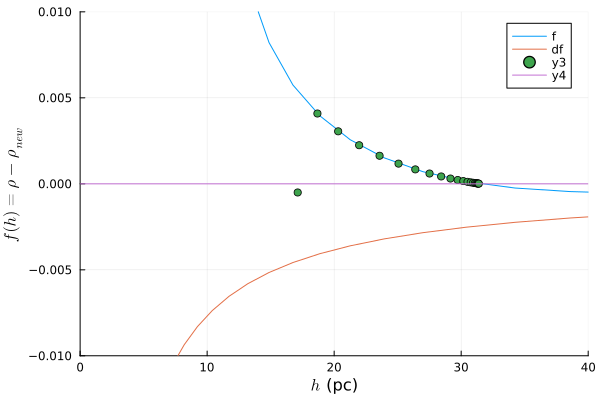
\includegraphics[width=\textwidth]{density.png}
\end{figure}

\newpage
\bibliographystyle{aasjournal}
\bibliography{background}

\end{document}
